% Figure snippets only. Not included by main.tex.
% Replace captured_20261123_082337 with the published folder name under figures/.

\begin{figure}[htbp]
\centering
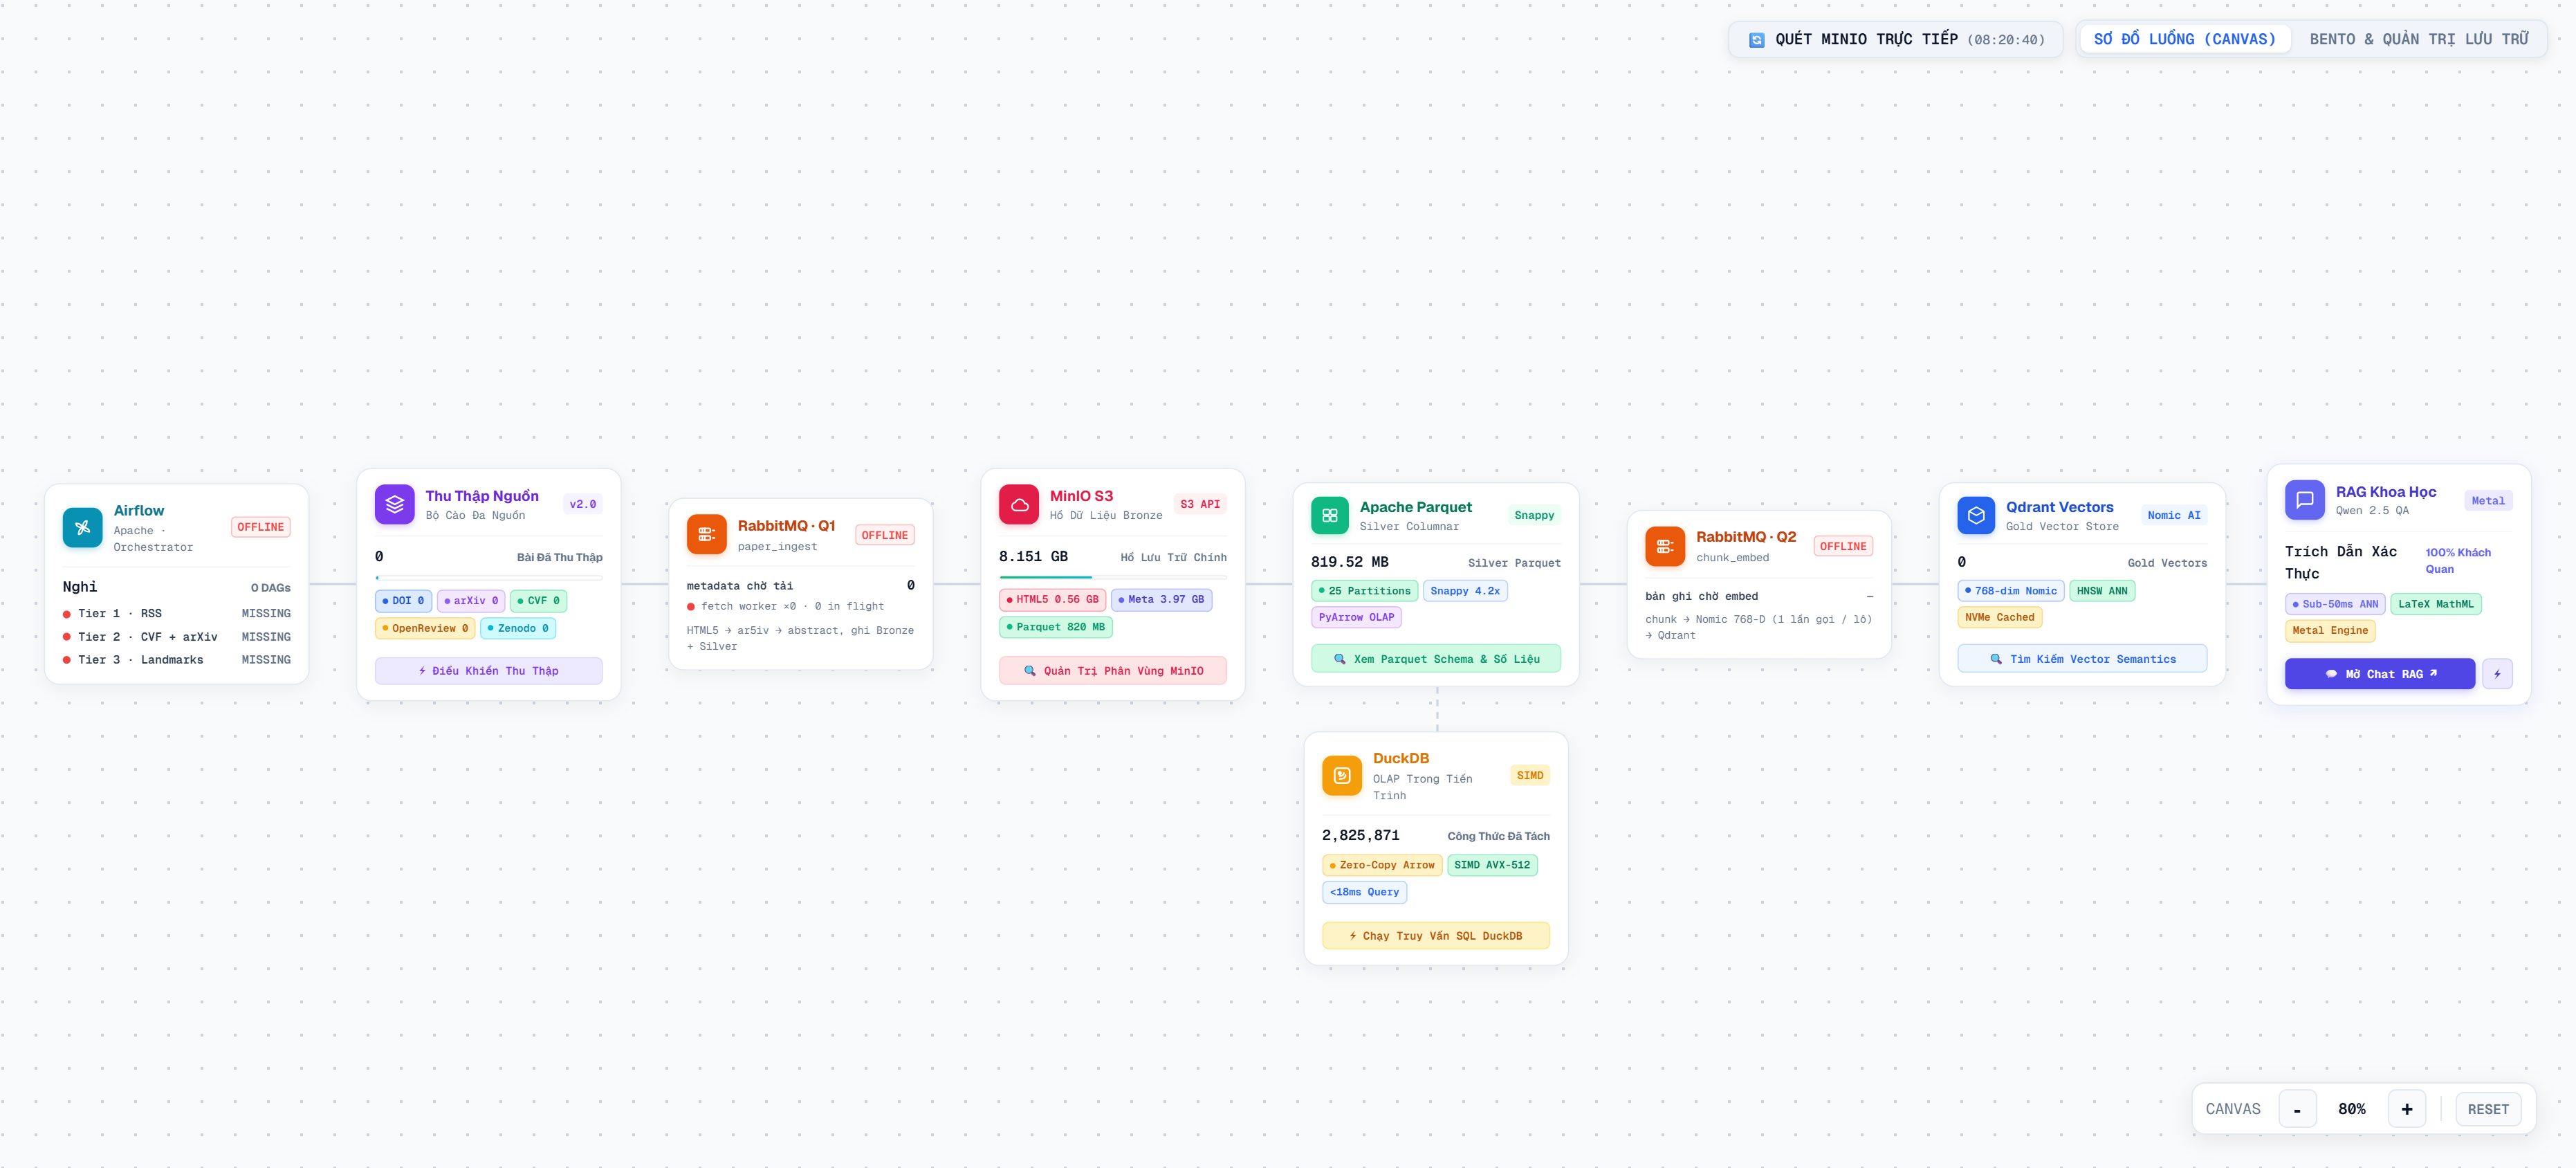
\includegraphics[width=\linewidth]{figures/captured_20261123_082337/01_pipeline_ui.png}
\caption[Giao diện sơ đồ luồng hai hàng đợi]{Giao diện sơ đồ luồng hai hàng đợi. Ảnh giao diện kiến trúc hiện tại. Airflow/RabbitMQ không hoạt động trong phiên chụp; Qdrant trả 502. Nhãn hiệu năng cố định trên canvas không phải kết quả benchmark. Không dùng ảnh để khẳng định toàn hệ thống đang vận hành.}
\label{fig:capture-01}
\end{figure}

\begin{figure}[htbp]
\centering
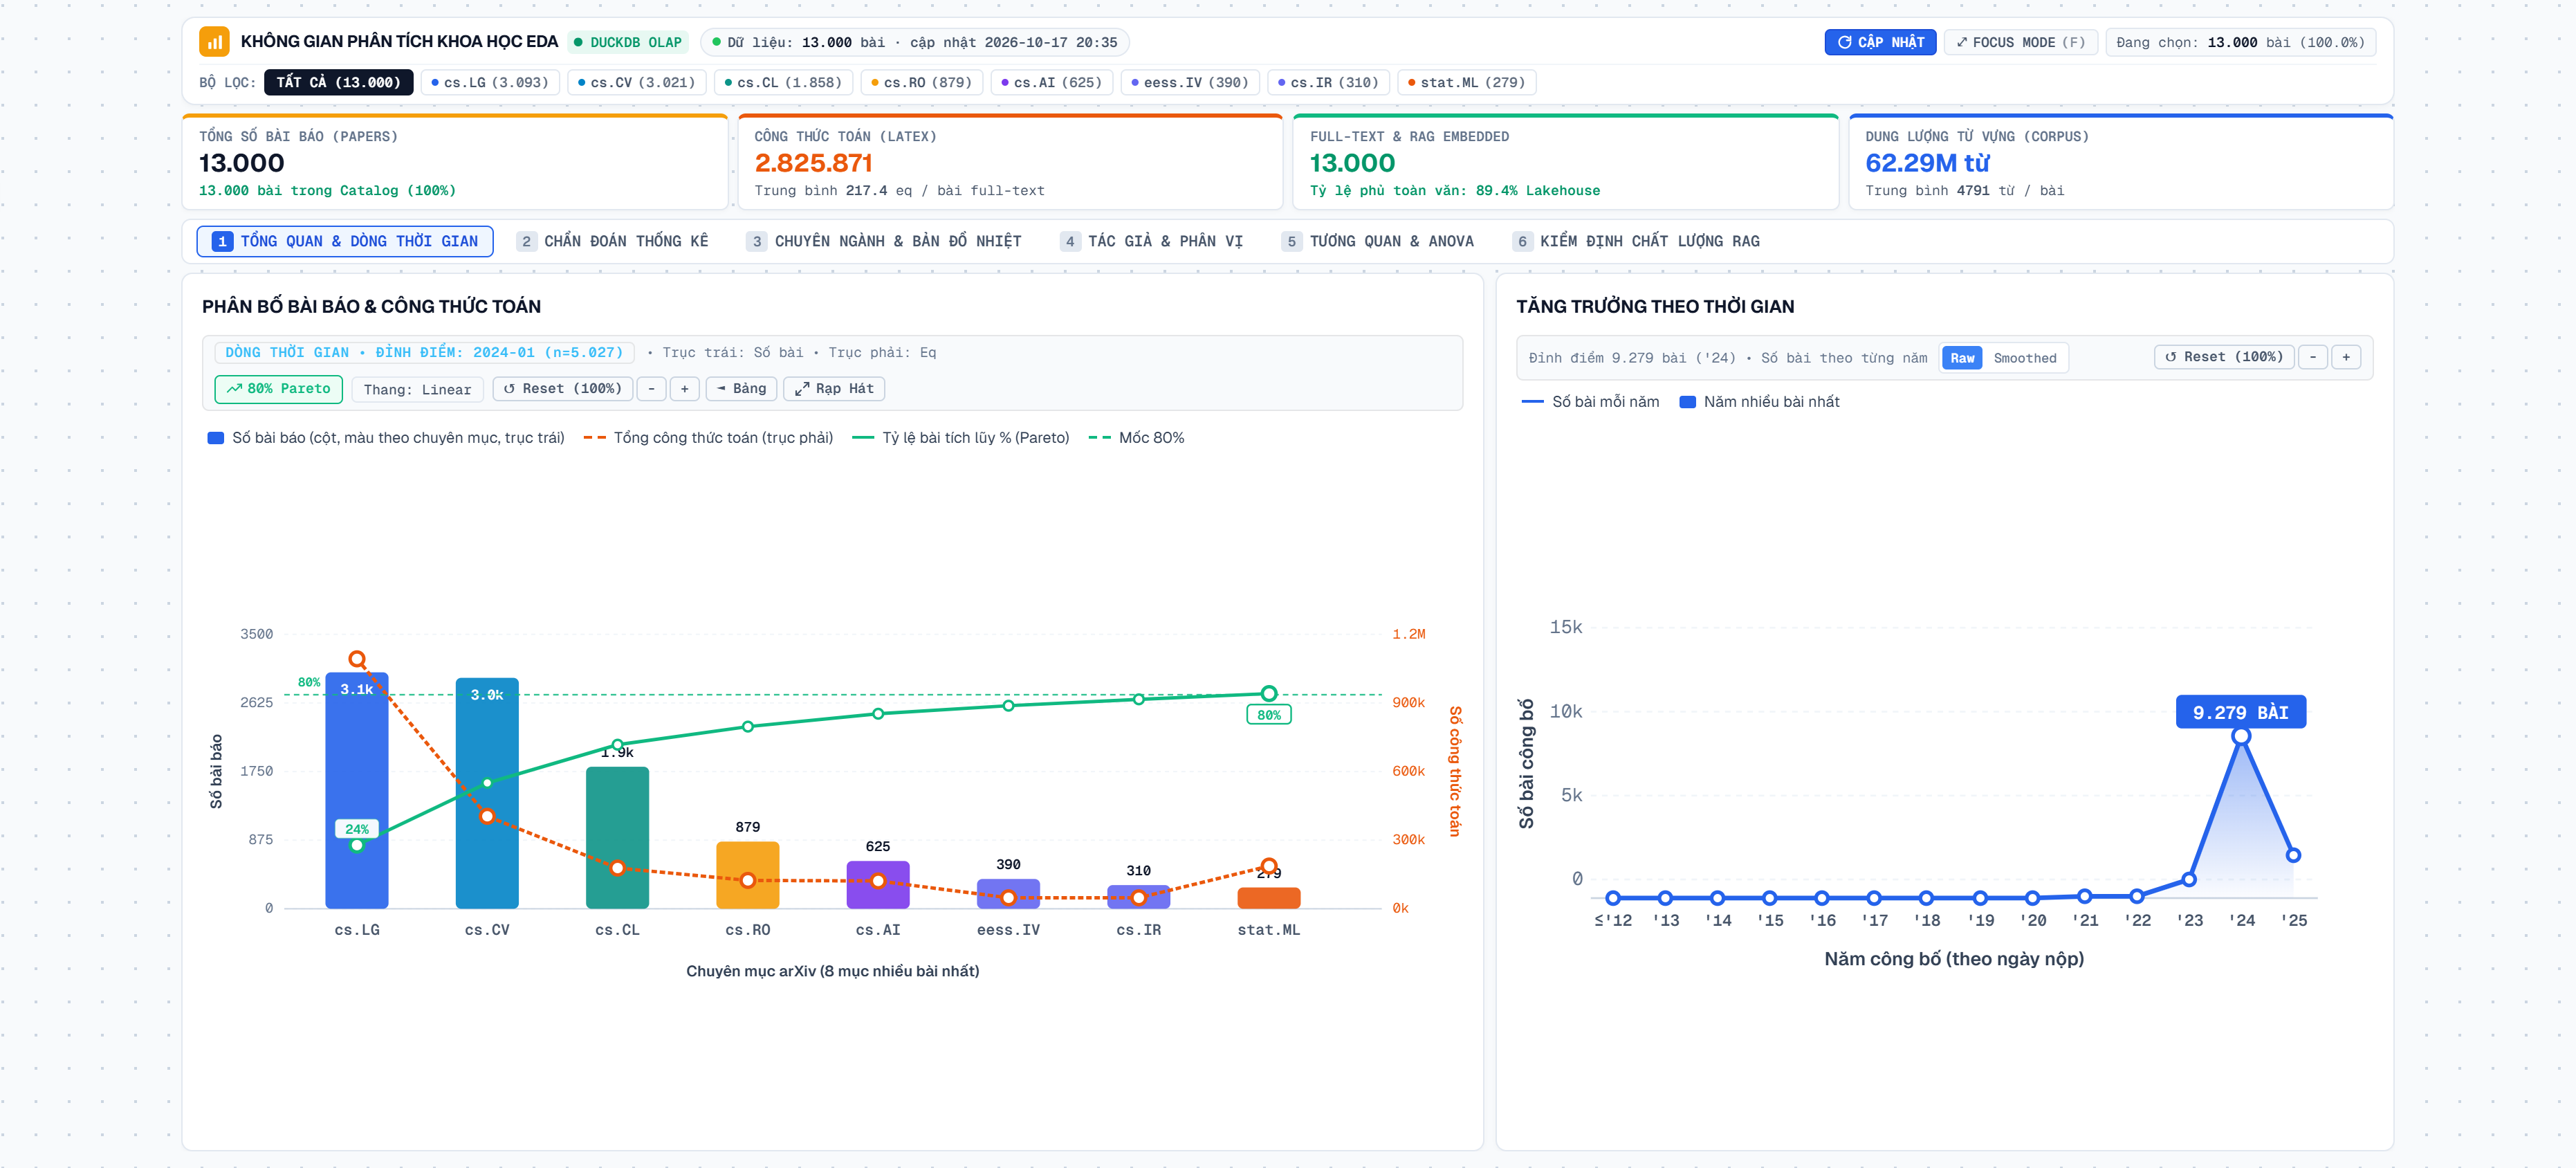
\includegraphics[width=\linewidth]{figures/captured_20261123_082337/03_eda_silver_overview.png}
\caption[EDA Silver: phân bố chuyên ngành và thời gian]{EDA Silver: phân bố chuyên ngành và thời gian. Dữ liệu artifact EDA lưu ngày 17/10/2026: 13.000 bài, 2.825.871 công thức. Đây là ảnh chụp mới của kết quả đã lưu; không phải lần chạy lại EDA hôm nay.}
\label{fig:capture-03}
\end{figure}

\begin{figure}[htbp]
\centering
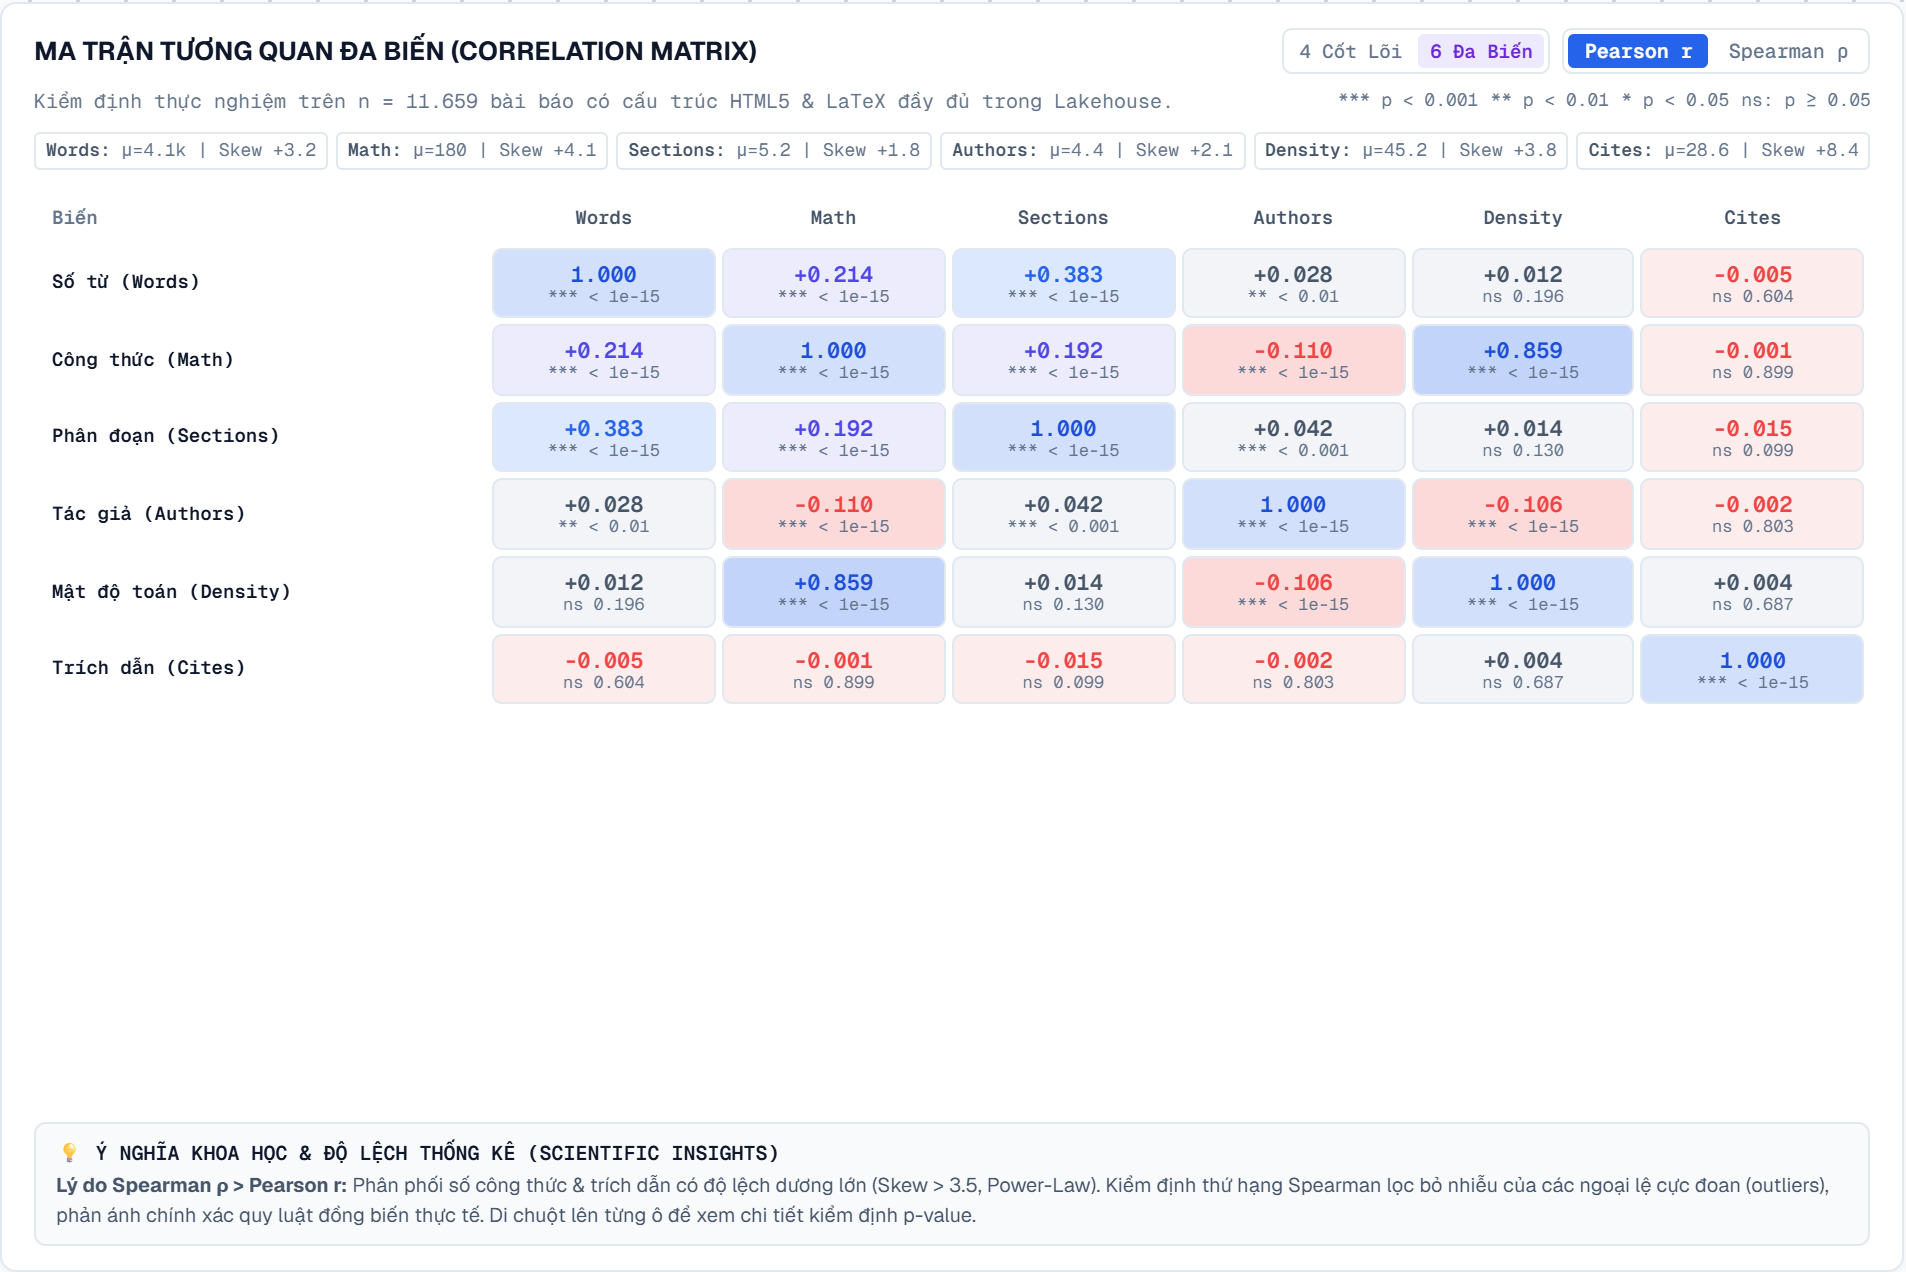
\includegraphics[width=\linewidth]{figures/captured_20261123_082337/04_pearson_correlation.png}
\caption[Ma trận tương quan Pearson r]{Ma trận tương quan Pearson r. Ma trận và p-value lấy từ artifact EDA đã lưu ngày 17/10/2026. Chỉ chụp panel ma trận; loại panel ANOVA bên cạnh vì các số ANOVA đang được viết cố định trong frontend. Các lời diễn giải vẫn cần đối chiếu hệ số.}
\label{fig:capture-04}
\end{figure}

\begin{figure}[htbp]
\centering
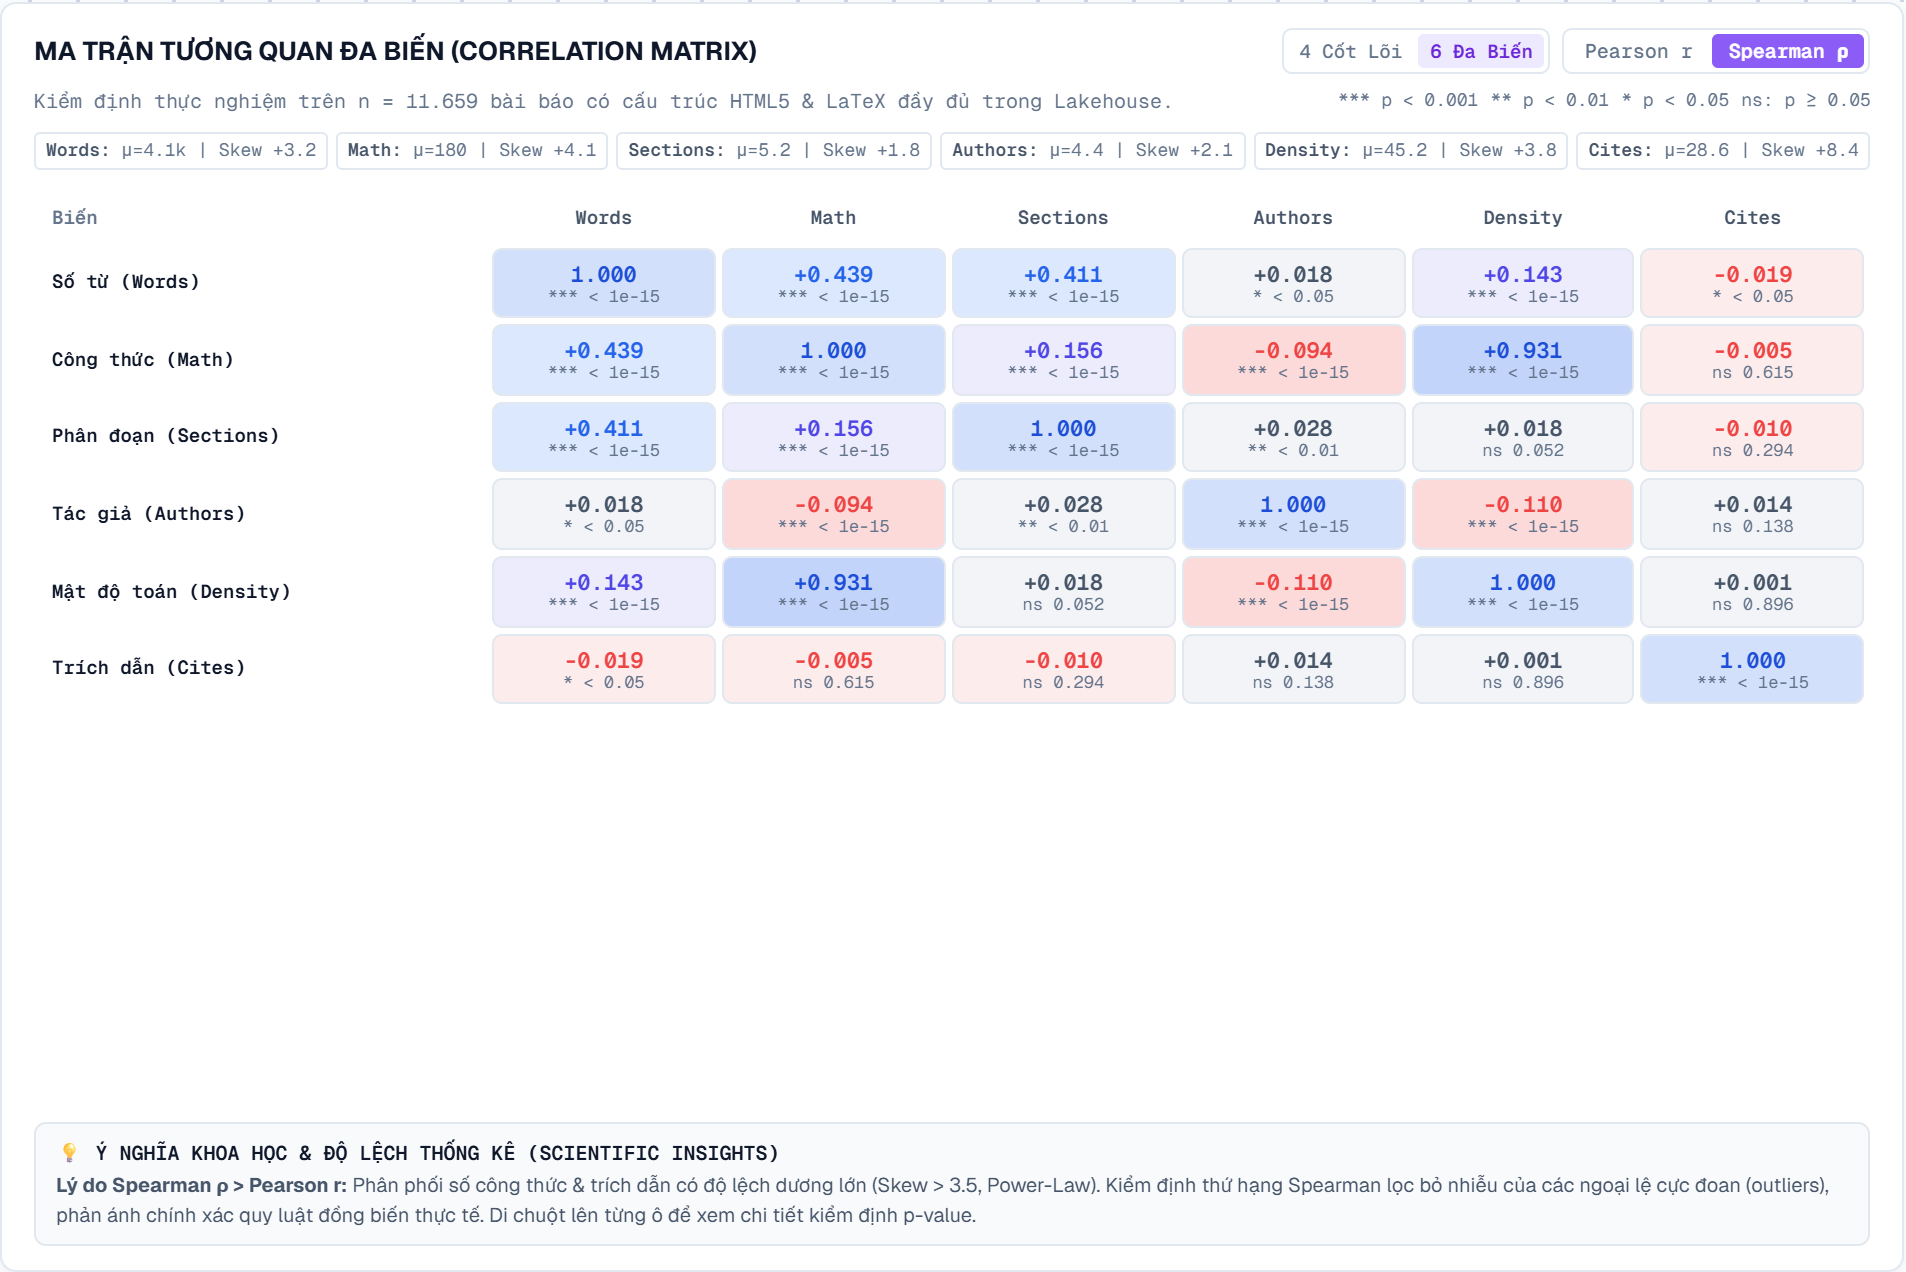
\includegraphics[width=\linewidth]{figures/captured_20261123_082337/05_spearman_correlation.png}
\caption[Ma trận tương quan Spearman ρ]{Ma trận tương quan Spearman ρ. Ma trận và p-value lấy từ artifact EDA đã lưu ngày 17/10/2026. Chỉ chụp panel ma trận; loại panel ANOVA bên cạnh vì các số ANOVA đang được viết cố định trong frontend. Các lời diễn giải vẫn cần đối chiếu hệ số.}
\label{fig:capture-05}
\end{figure}

\begin{figure}[htbp]
\centering
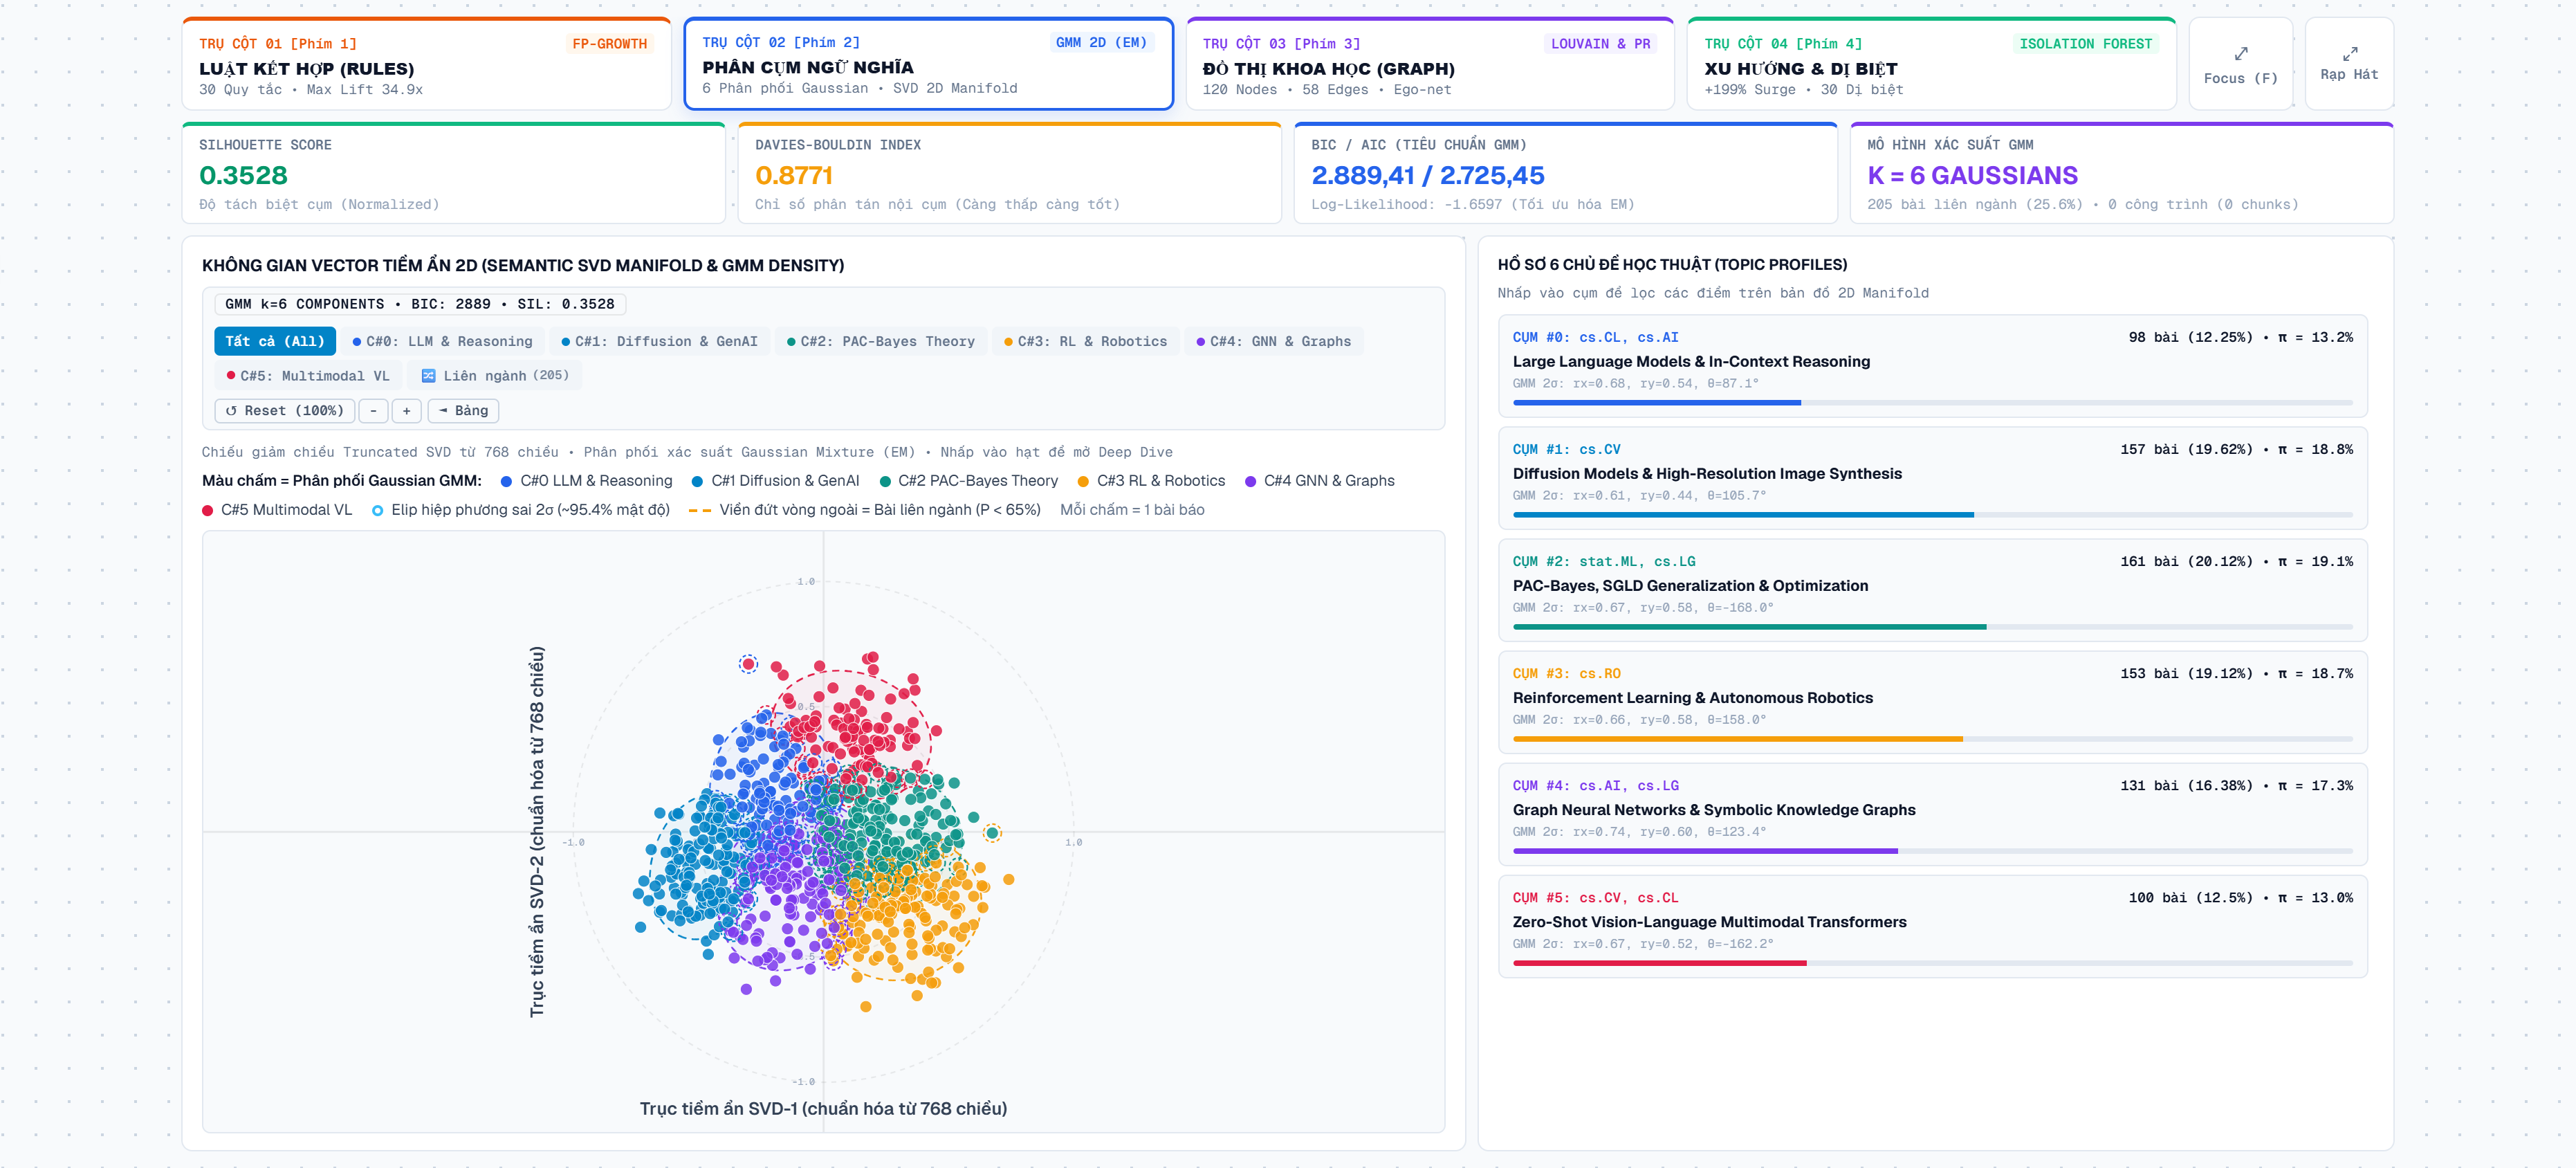
\includegraphics[width=\linewidth]{figures/captured_20261123_082337/06_gmm_clusters.png}
\caption[GMM: không gian cụm từ artifact đã lưu]{GMM: không gian cụm từ artifact đã lưu. Artifact GMM lưu ngày 20/10/2026, 800 mẫu, K=6. UI vẫn ghi SVD và có các nhãn chủ đề cố định; ảnh không xác minh pipeline PCA hiện tại hoặc tính đúng của tên chủ đề.}
\label{fig:capture-06}
\end{figure}

\begin{figure}[htbp]
\centering
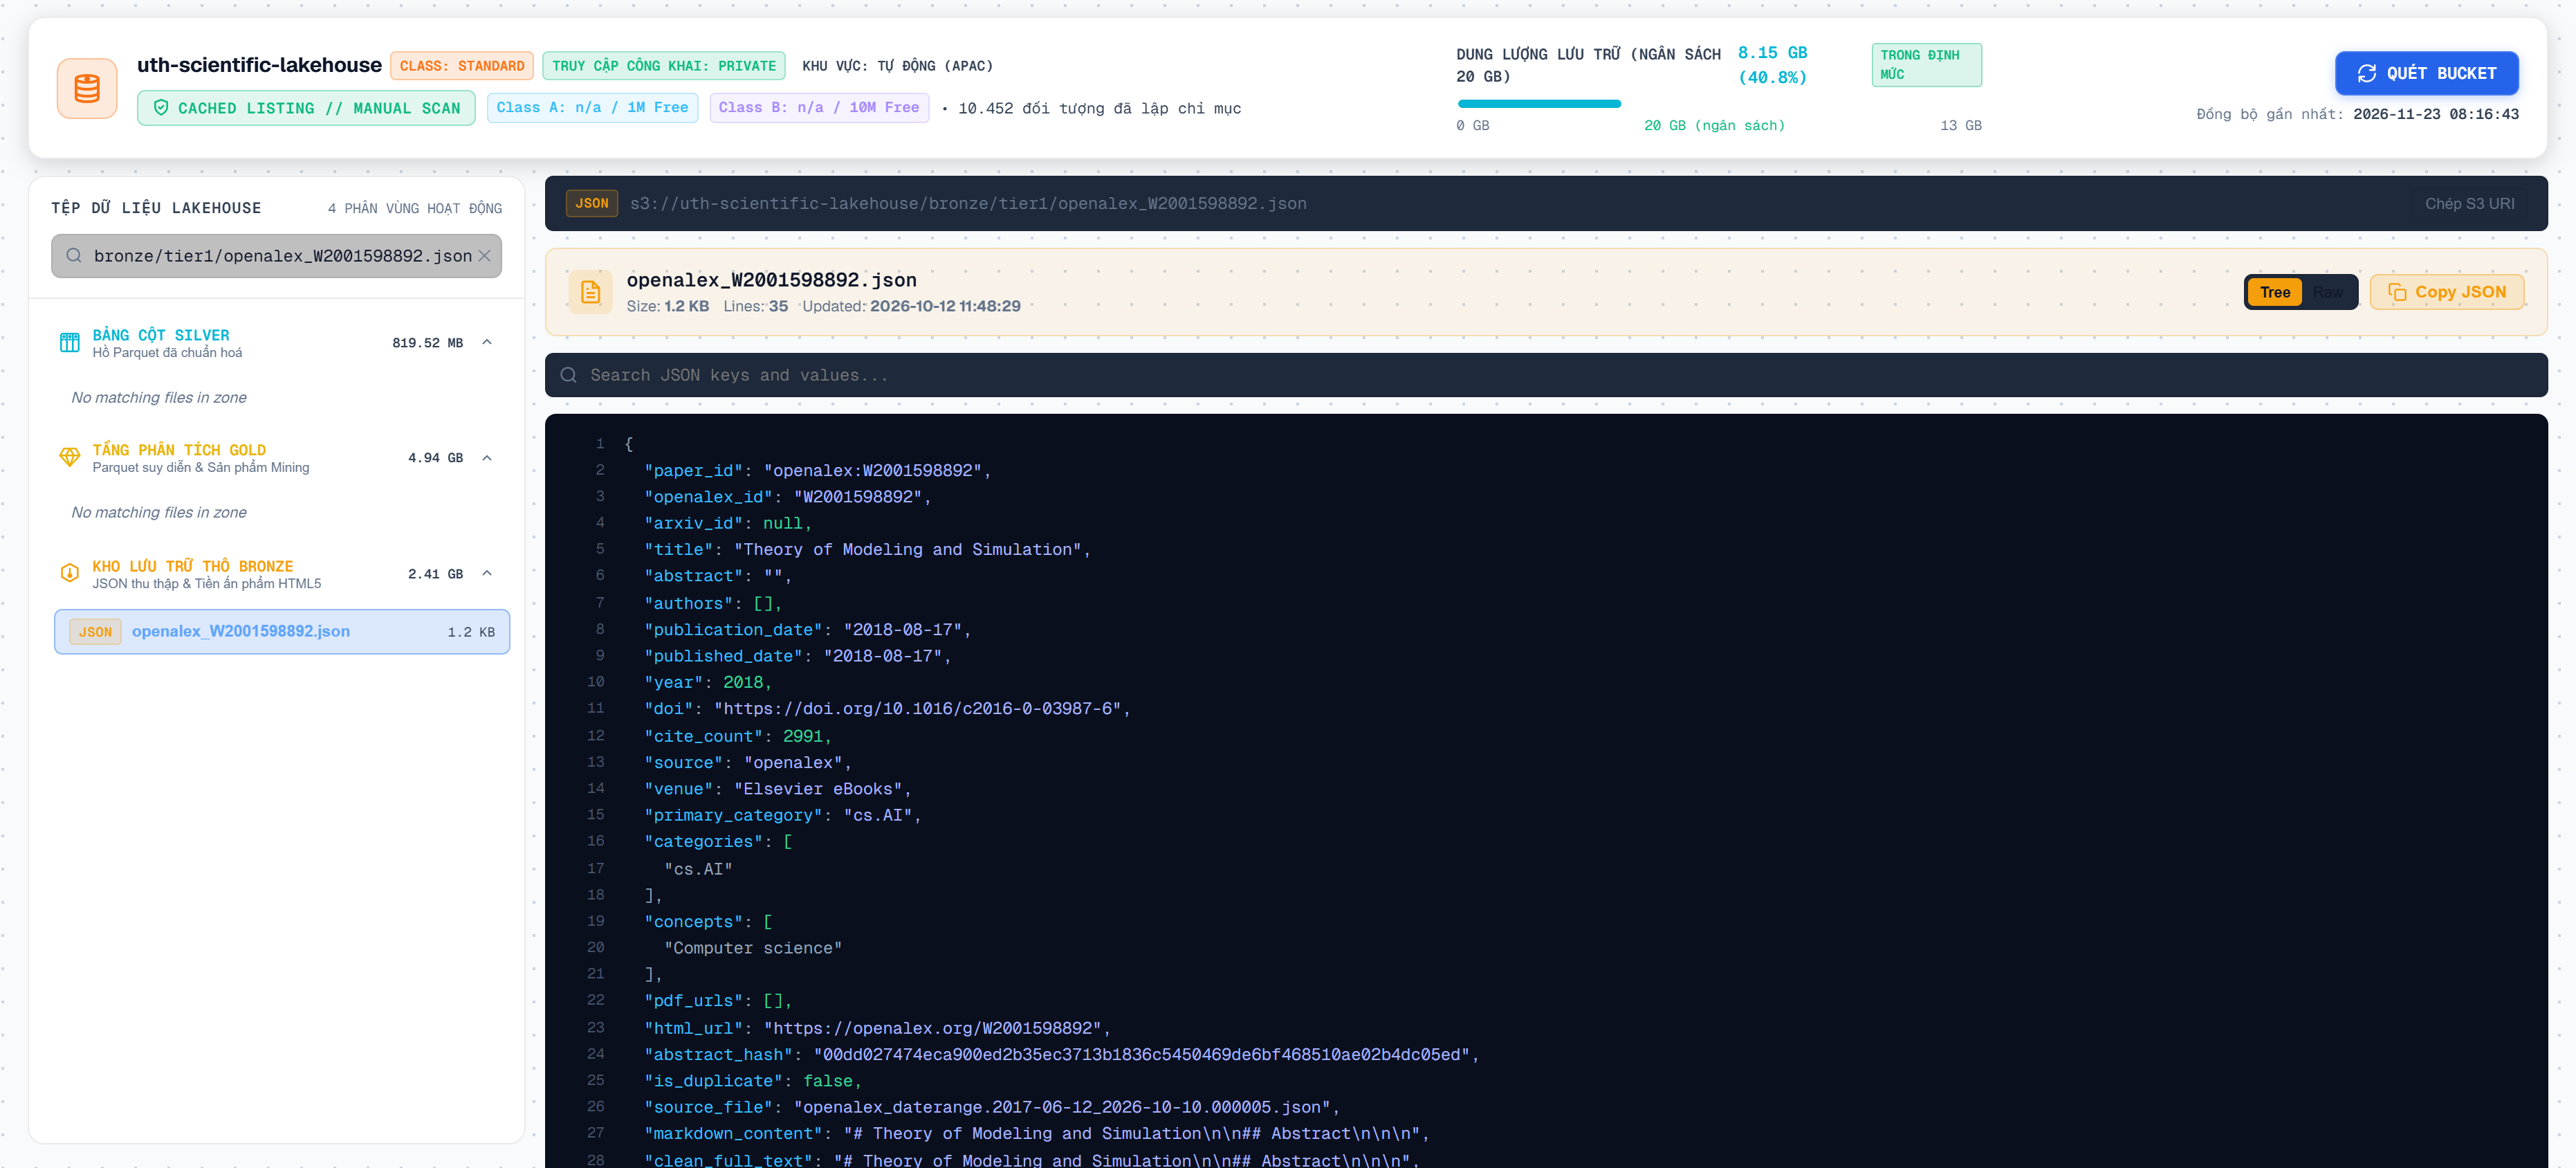
\includegraphics[width=\linewidth]{figures/captured_20261123_082337/02_bronze_raw_metadata.png}
\caption[Ví dụ bản ghi metadata thô Bronze]{Ví dụ bản ghi metadata thô Bronze. Ví dụ một bản ghi thực đọc từ kho; đây là minh chứng cấu trúc raw metadata, không phải thống kê EDA Bronze. Không suy ra số bài từ số object trong Explorer.}
\label{fig:capture-02}
\end{figure}

\begin{figure}[htbp]
\centering
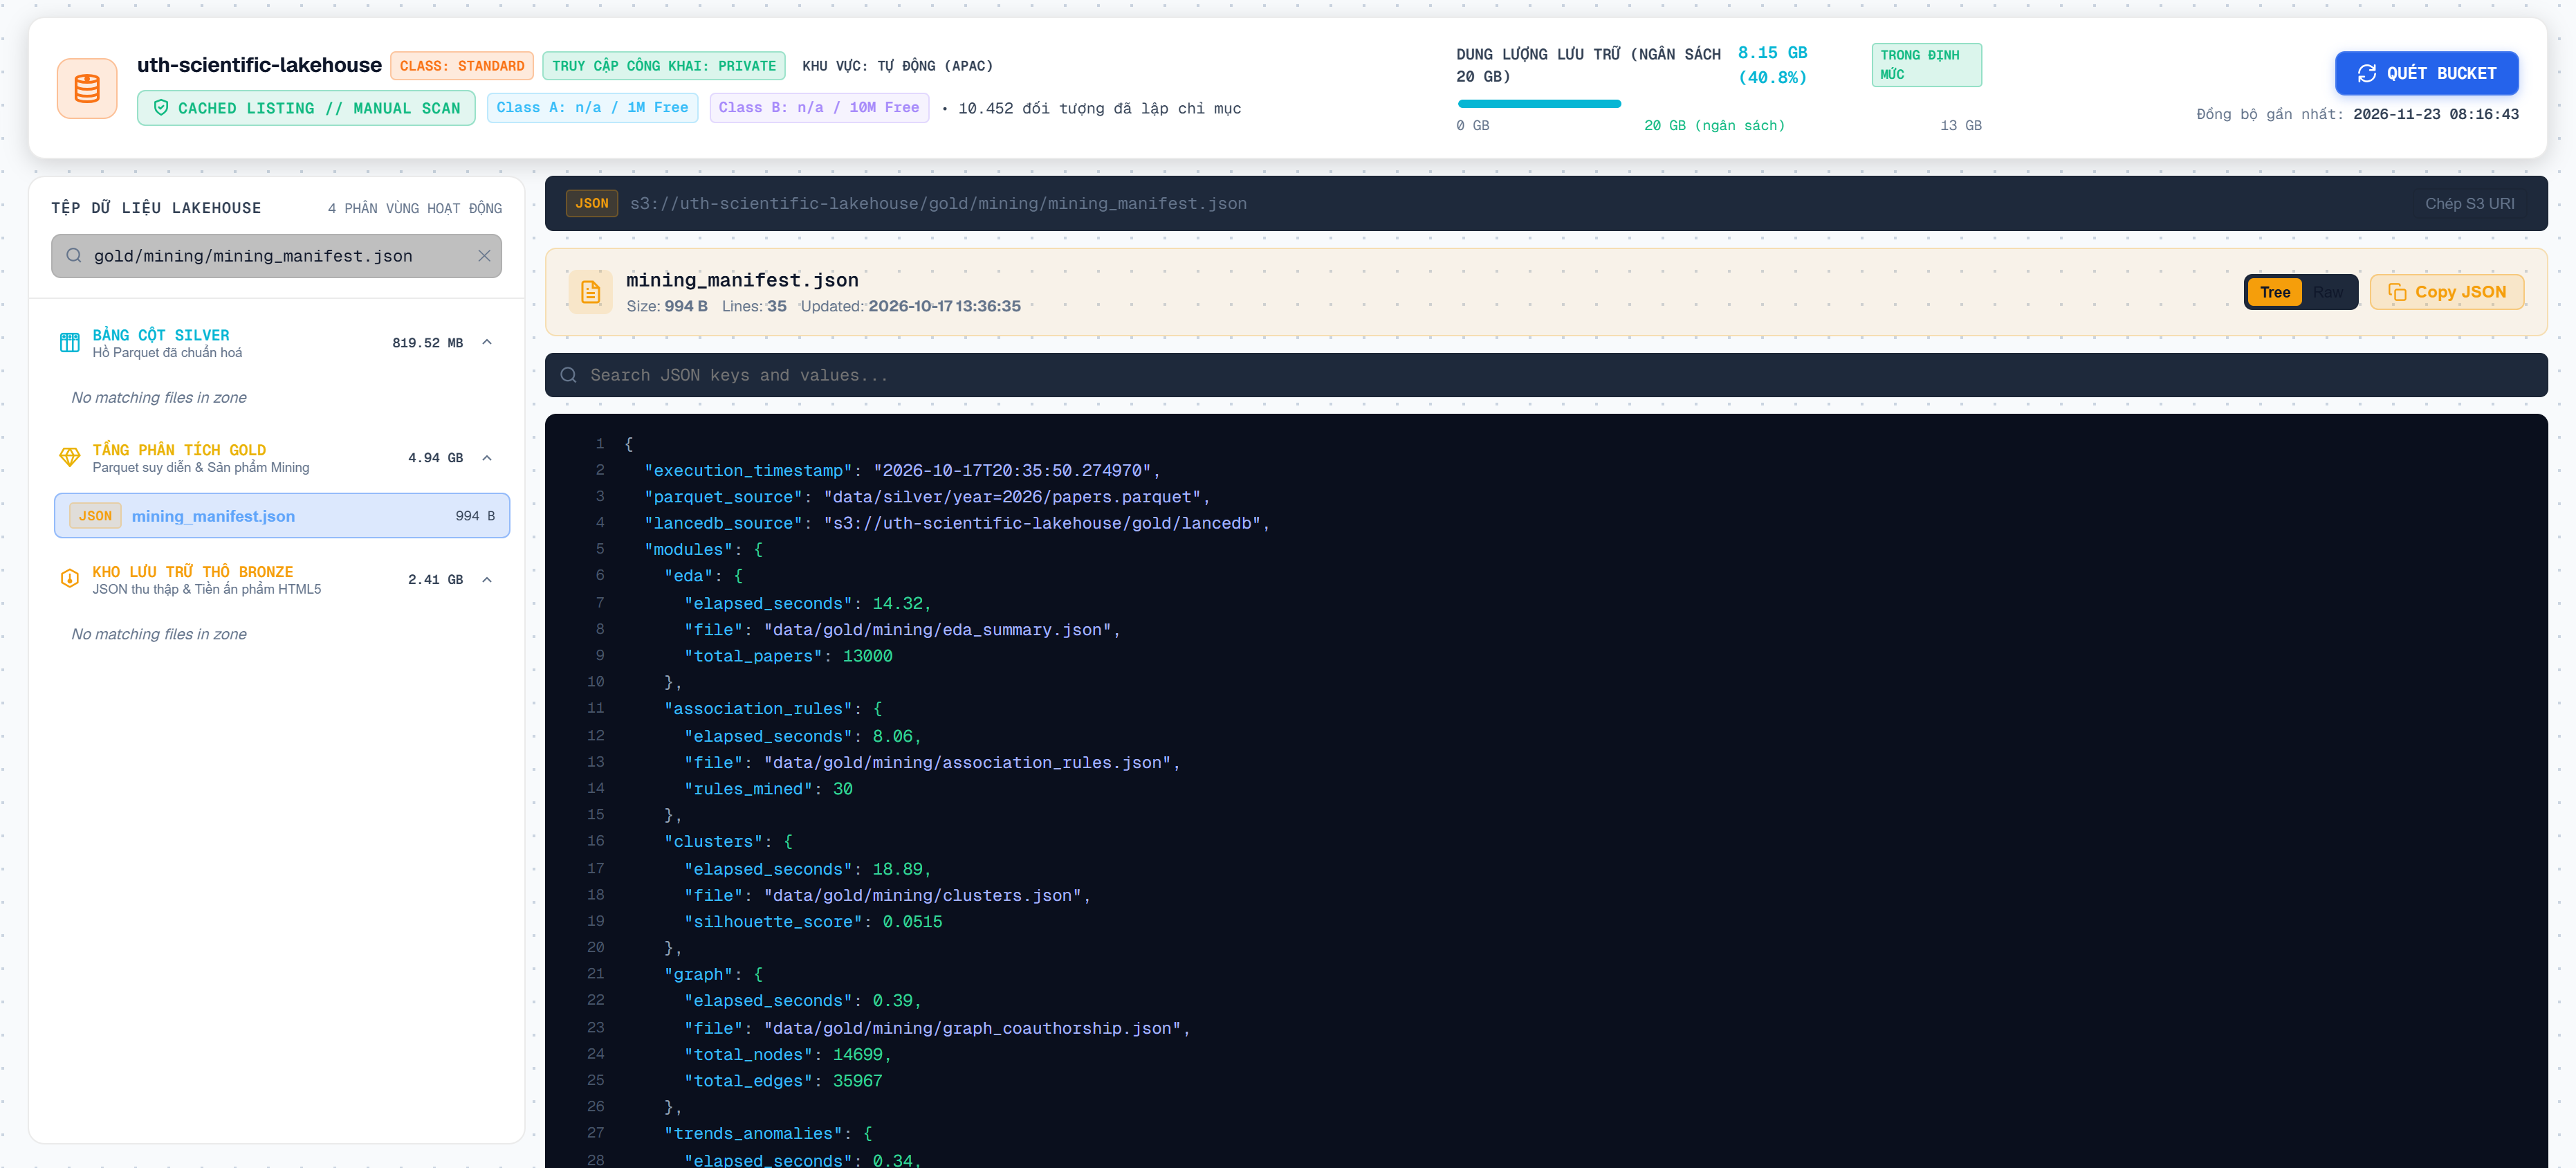
\includegraphics[width=\linewidth]{figures/captured_20261123_082337/07_gold_mining_manifest.png}
\caption[Manifest sản phẩm khai phá Gold]{Manifest sản phẩm khai phá Gold. Manifest lịch sử trên kho Gold. Trường lancedb\_source phản ánh kiến trúc tại lần chạy cũ; không phải xác nhận trạng thái Qdrant hiện tại.}
\label{fig:capture-07}
\end{figure}
